% -*- mode: fundamental -*-

% Slides accompanying "Learn RISC-V CPU Implementation and BSV" book
% Copyright (c) 2024 Rishiyur S. Nikhil, All Rights Reserved

% -*- mode: fundamental -*-

% Slides accompanying "Learn RISC-V CPU Implementation and BSV" book
% Copyright (c) 2024 Rishiyur S. Nikhil, All Rights Reserved

% This is a preamble shared by all the slide decks

\documentclass[10pt, aspectratio=169]{beamer}

% \documentclass[17pt]{beamer}

% Avail. font sizes: 8pt, 9pt, 10pt, 11pt, 12pt, 14pt, 17pt, 20pt.
% Default font size is 11pt (= 22pt in full screen mode).

\usepackage{verbatim}
\usepackage{fancyvrb}
\usepackage{listings}

% ================================================================
% Themes

\usetheme{Madrid}          % Line at bottom: Author (affiliation), OptTitle, Conf, page 

% \usetheme{Copenhagen}    % Same as Madrid except bottom line: Author, OptTitle

% \usetheme{Berkeley}    % Takes up 1-inch border on left and top

% ----------------
% colorthemes
% (default), beaver, beetle, seahorse, wolverine

\usecolortheme{seahorse}

% ================================================================
% Customization: show table of contents before each section
% Use \AtBeginSubsection    to show before each subsection

% \AtBeginSection[]
% {
%   \begin{frame}
%     \frametitle{Table of Contents}
%     \tableofcontents[currentsection]
%   \end{frame}
% }

% ================================================================

% ----------------
% The bsc compiler and BSV language
\newcommand{\bsc}{\emph{bsc}}
\newcommand{\BSV}{\bf{BSV}}
% ----------------
% ITALICISE WORDS
\newcommand{\ie}{\emph{i.e.,}}
\newcommand{\eg}{\emph{e.g.,}}
\newcommand{\Eg}{\emph{E.g.,}}
\newcommand{\etc}{\emph{etc.}}
\newcommand{\via}{\emph{via}}
\newcommand{\vs}{\emph{vs.}}

% ----------------
% EMPTY BOXES OF VARIOUS WIDTHS, FOR INDENTATION

\newcommand{\hm}{\hspace*{1em}}
\newcommand{\hmm}{\hspace*{2em}}
\newcommand{\hmmm}{\hspace*{3em}}
\newcommand{\hmmmm}{\hspace*{4em}}

% ----------------
% Convenient widths

\newlength{\hlessmm}
\setlength{\hlessmm}{\textwidth}
\addtolength{\hlessmm}{-2em}

\newlength{\hlessmmm}
\setlength{\hlessmmm}{\textwidth}
\addtolength{\hlessmmm}{-3em}

\newlength{\hlessmmmm}
\setlength{\hlessmmmm}{\textwidth}
\addtolength{\hlessmmmm}{-4em}

% ================================================================
% Title page

\title[Learn CPU design \& BSV]{Learn RISC-V CPU Implementation and BSV}

\subtitle{(BSV: a High-Level Hardware Design Language)}

\author[{\copyright} R.S.Nikhil]{Rishiyur S.~Nikhil}
% \institute{Bluespec, Inc.}

% Date is set differently in each slide deck

% \logo{
\includegraphics[height=0.6cm]{../Figures/Bluespec_Logo_2022-10}}

% End of preamble
% ****************************************************************


\date{L3: Structure of BSV Programs}

% ****************************************************************

\begin{document}

% ================================================================

\begin{frame}
 \titlepage

 \begin{center}
  
\includegraphics[height=1cm]{../Figures/Bluespec_Logo_2022-10}
 \end{center}
\end{frame}

% ================================================================

\begin{frame}
\frametitle{BSV language, compiler and libraries documents}

From the book, Appendix A.6.5:

\fbox{\footnotesize
\hm
\begin{minipage}{\hlessmm}
\begin{itemize}

  \item The ``{\BSV} Language Reference
  Guide''.  This document describes the
  syntax and semantics of {\BSV}.

  PDF: \url{https://github.com/B-Lang-org/bsc/releases/latest/download/BSV_lang_ref_guide.pdf}

  \vspace*{1ex}

  \item The ``BSC Libraries Reference
  Guide''.  This document describes the
  extensive set of libraries and IP (Intellectual Property blocks)
  available to the {\BSV} user.

  PDF: \url{https://github.com/B-Lang-org/bsc/releases/latest/download/bsc_libraries_ref_guide.pdf}

  \vspace*{1ex}

  \item The ``BSC User Guide''.  This document
  describes how to use the {\bsc} compiler, which compiles our
  hardware descriptions written in {\BSV} into Verilog (which can then
  be simulated or synthesizes using standard Verilog tools).

  PDF: \url{https://github.com/B-Lang-org/bsc/releases/latest/download/bsc_user_guide.pdf}

\end{itemize}

\vspace*{1ex}

We will be using the Language Reference Guide and Librares Reference
Guide extensively, so you may wish to download a copy for your laptop.
\end{minipage}}


\end{frame}

% ================================================================

\begin{frame}
\frametitle{\EmojiExercise \hmm Exercise break}

A minimal (trivial!) {\BSV} program.

\vspace{2ex}

Please see directory {\tt Ex\_O3\_A}, code and {\tt Makefile}.

\vspace{5ex}

{\tt README.txt} and the code contain notes and suggested variations.

\vspace{1ex}

(More related exercises in the book, Chapter 3.)

\end{frame}

% ================================================================

\begin{frame}
\frametitle{File-level view of a BSV program}

\begin{center}
\includegraphics[width=\textwidth]{../Figures/Fig_BSV_program_structure}
\end{center}

\end{frame}

% ================================================================

\begin{frame}
\frametitle{What's in a BSV package/file?}

\begin{center}
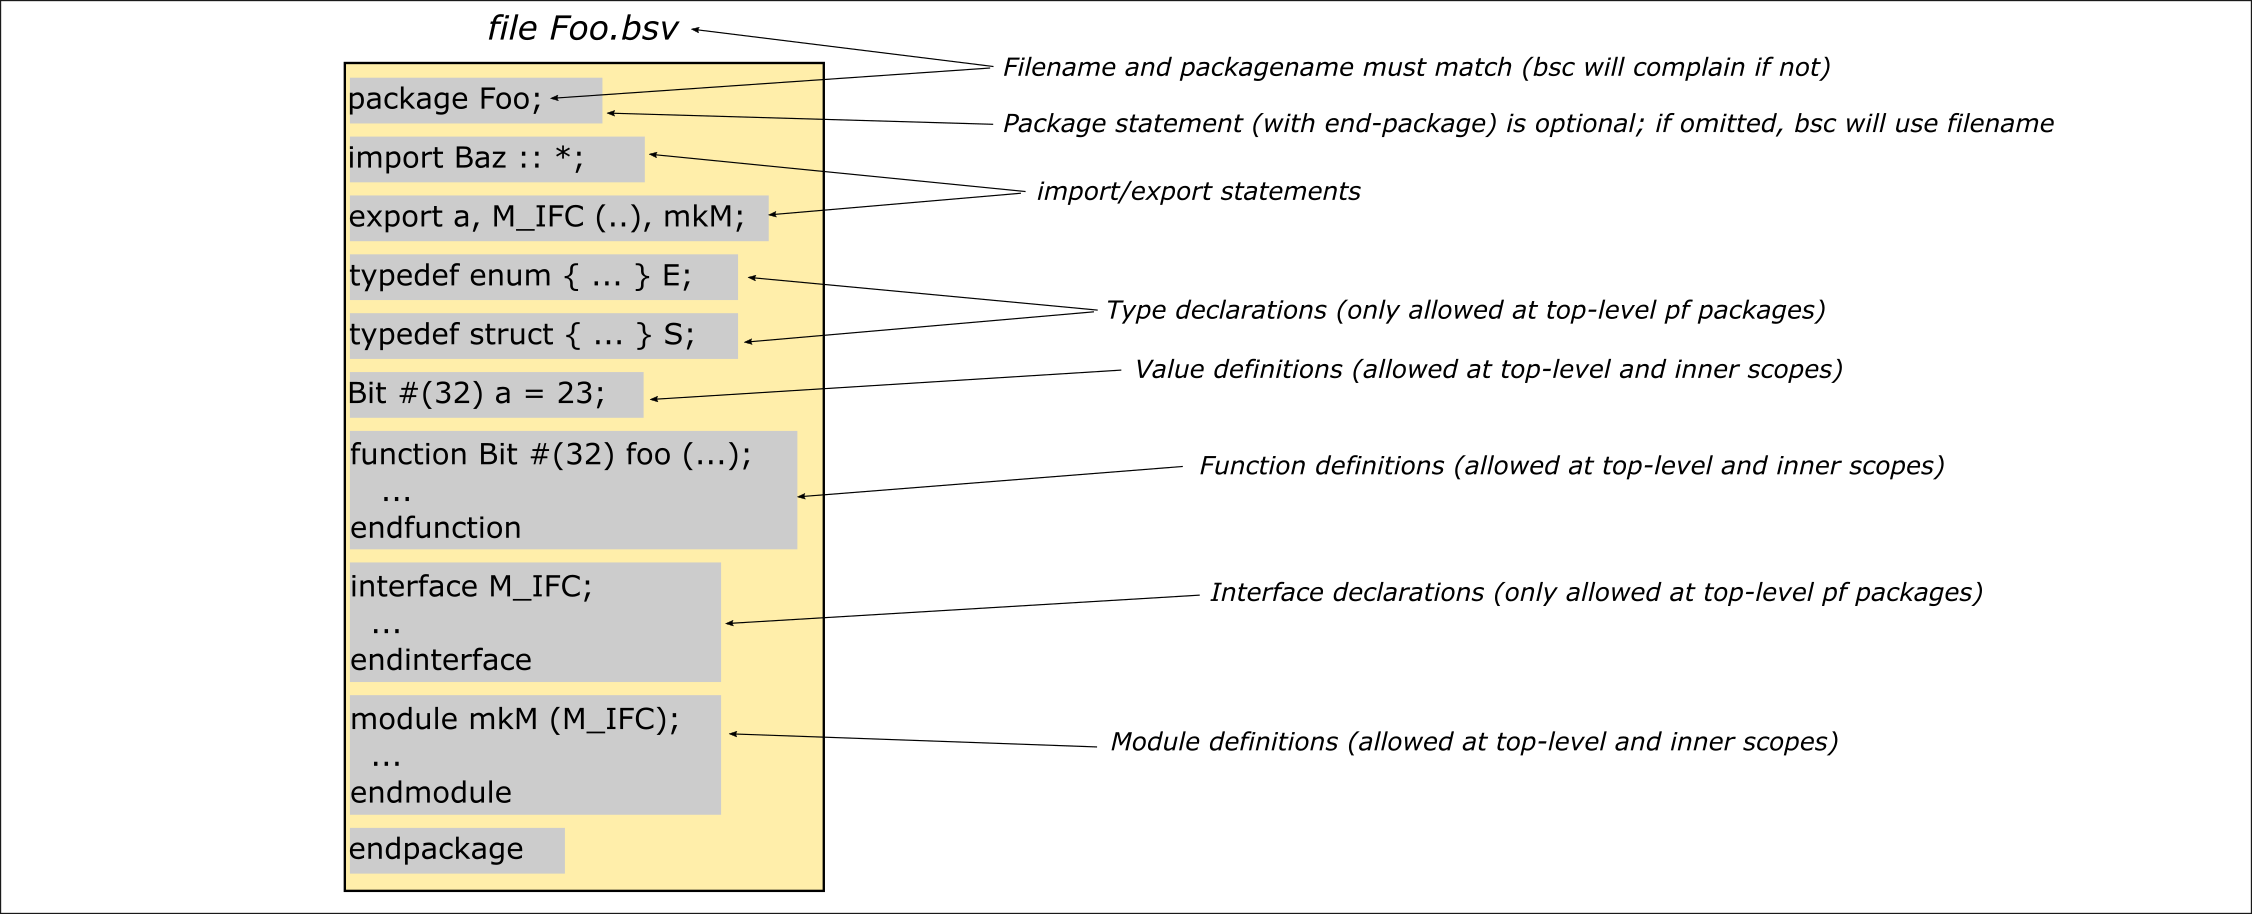
\includegraphics[width=\textwidth]{../Figures/Fig_BSV_Package}
\end{center}

\end{frame}

% ================================================================

\begin{frame}
\frametitle{Namespace control with package imports and exports}

\begin{center}
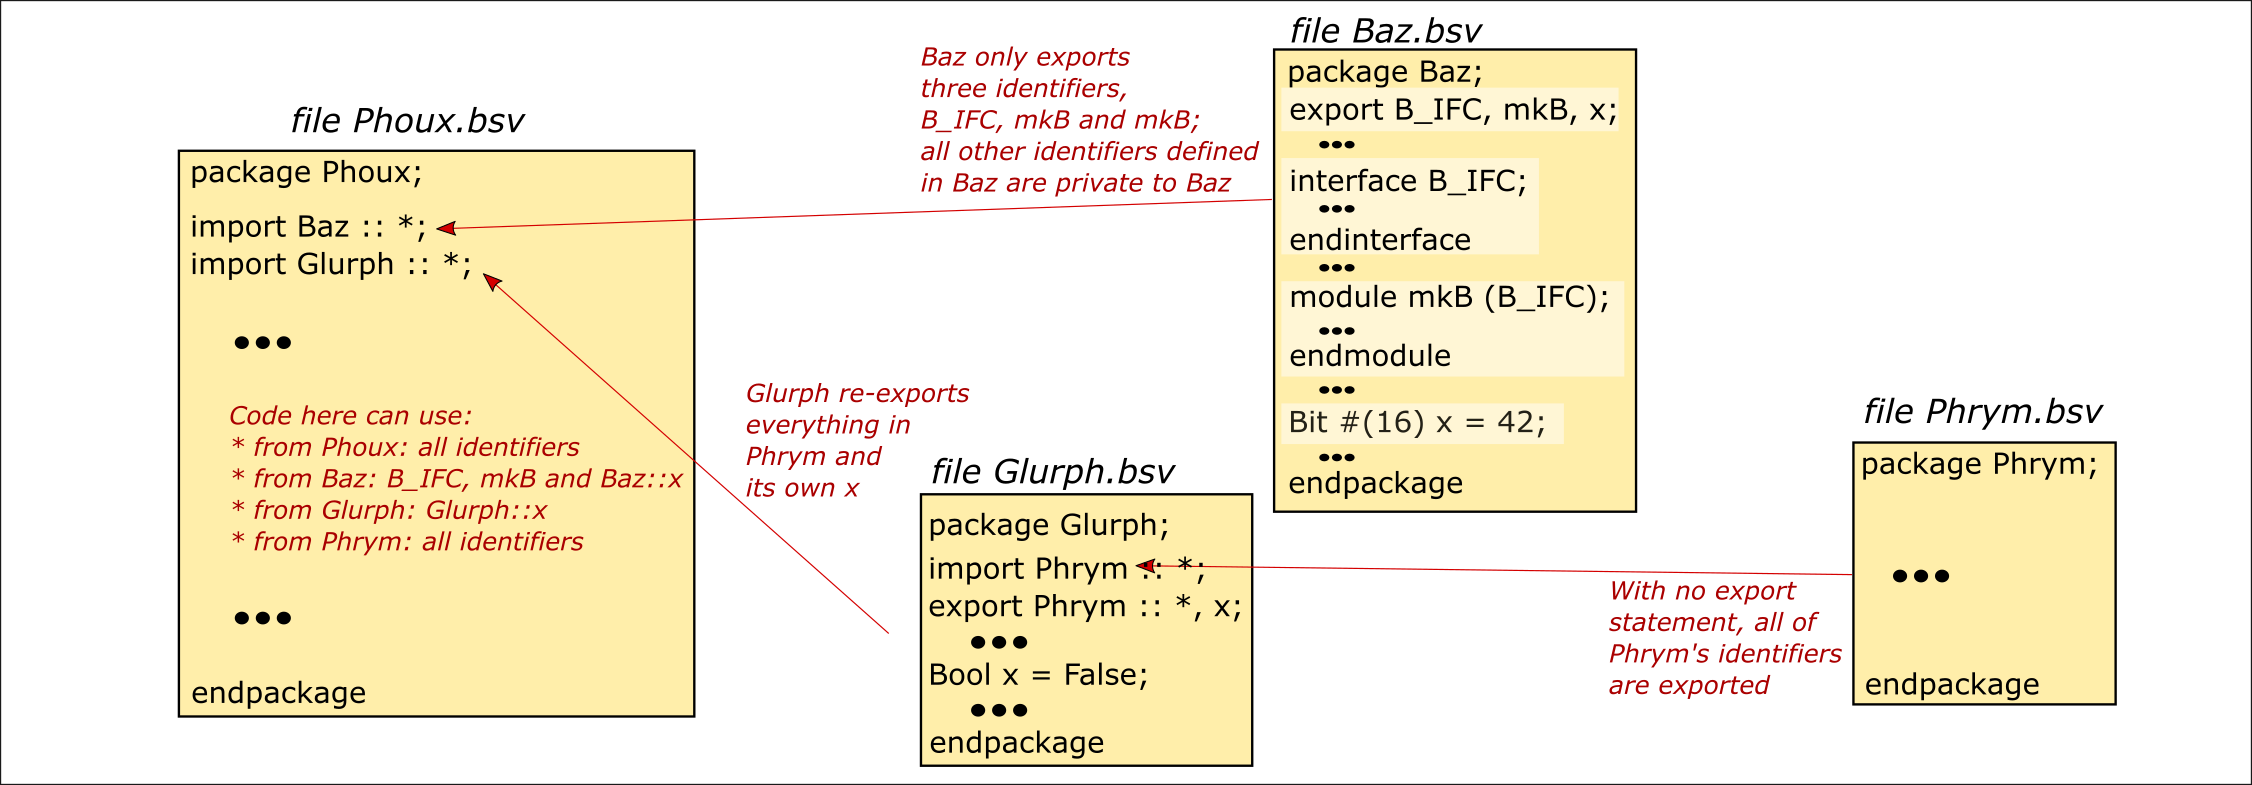
\includegraphics[width=\textwidth]{../Figures/Fig_BSV_namespace_control}
\end{center}

\end{frame}

% ================================================================

\begin{frame}
\frametitle{\EmojiExercise \hmm Exercise break}

Extending our Minimal BSV program to two packages/files.

\vspace{2ex}

Please see directory {\tt Ex\_O3\_B}, code and {\tt Makefile}.

\vspace*{5ex}

{\tt README.txt} and the code contain notes and suggested variations.

\vspace{1ex}

(More related exercises in the book, Chapter 3.)

\end{frame}

% ================================================================

\begin{frame}
\frametitle{What's in an Interface Declaration?}

\begin{center}
\includegraphics[width=\textwidth]{../Figures/Fig_BSV_whats_in_an_interface_decl}
\end{center}

\end{frame}

% ================================================================

\begin{frame}
\frametitle{What's in a Module Declaration?}

\begin{center}
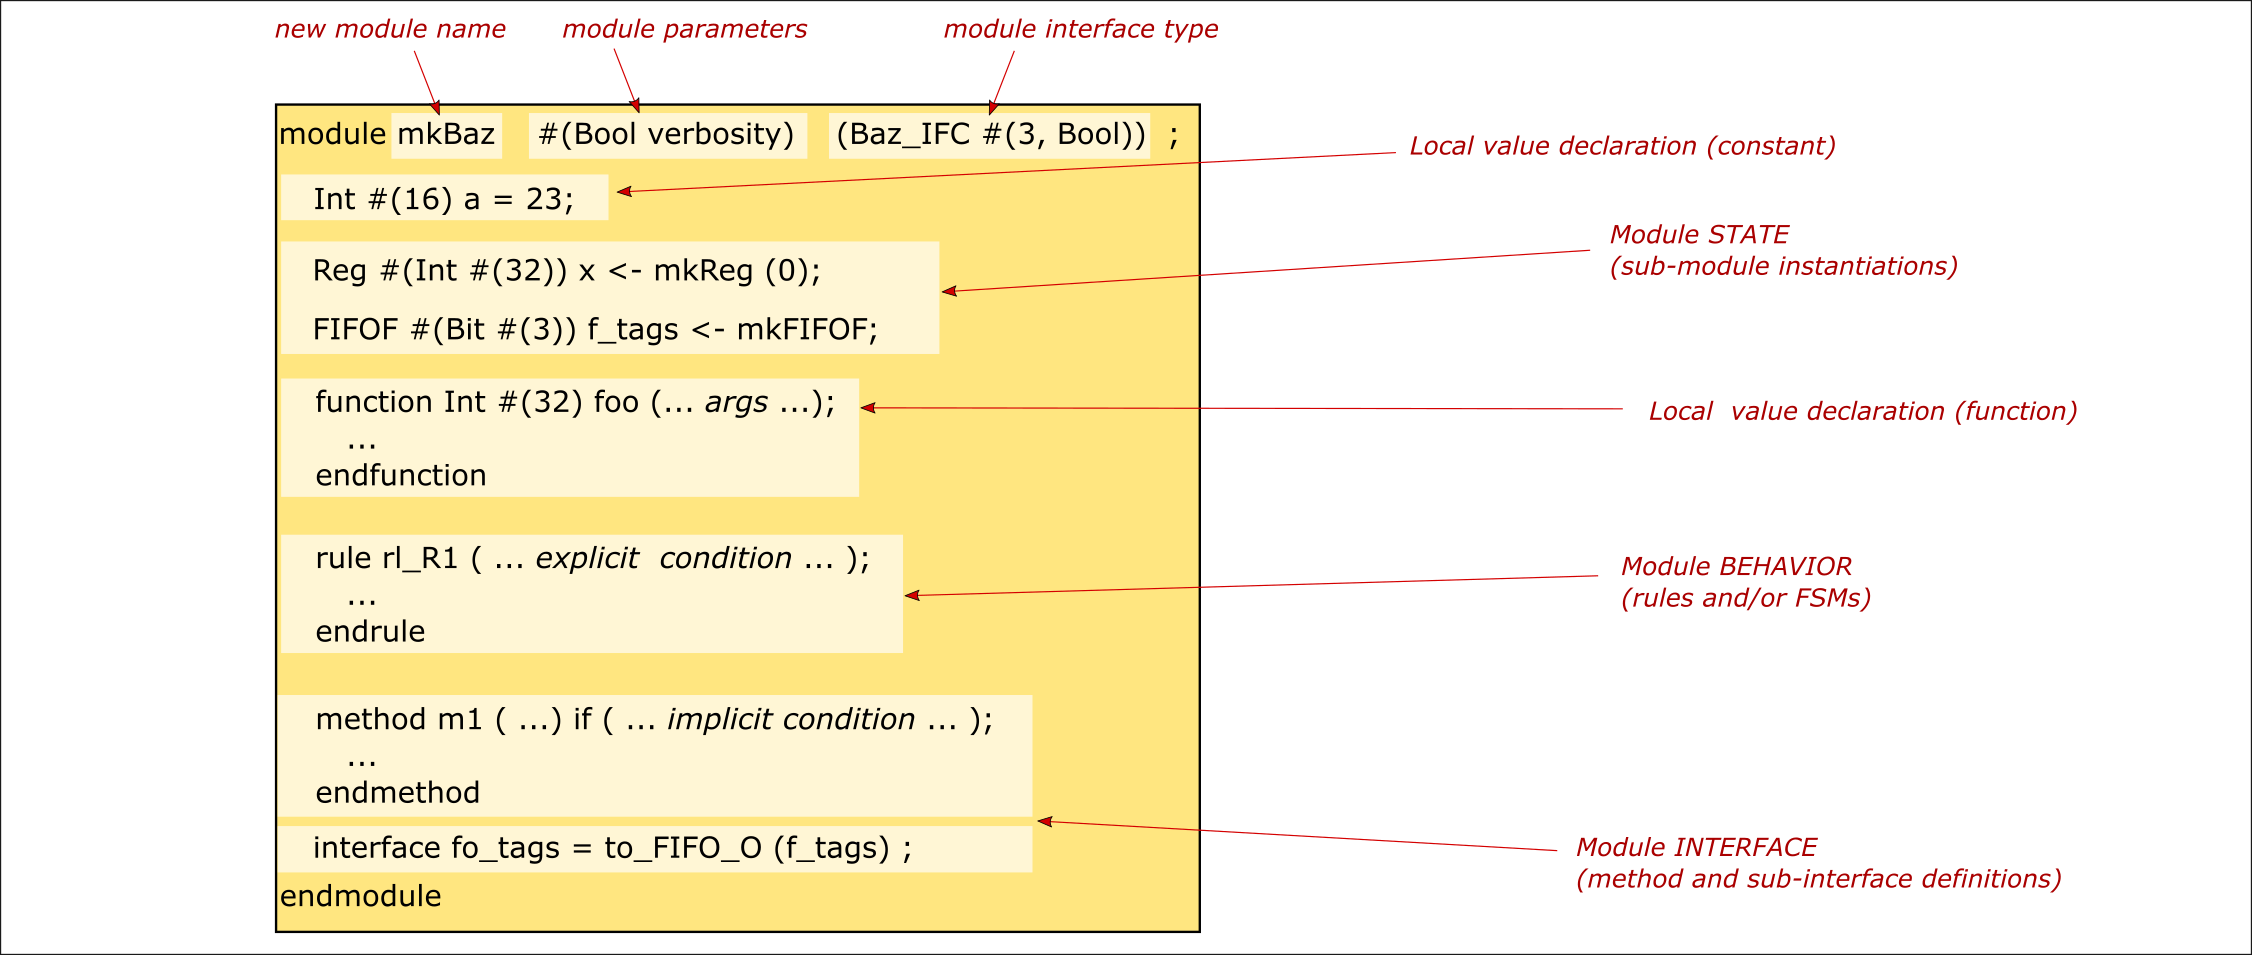
\includegraphics[width=\textwidth]{../Figures/Fig_BSV_whats_in_a_module_decl}
\end{center}

\end{frame}

% ================================================================

\begin{frame}
\frametitle{\EmojiExercise \hmm Exercise break}

Extending our minimal BSV program to define a module with an interface.

\vspace{2ex}

Please see directory {\tt Ex\_O3\_C}, code and {\tt Makefile}.

\vspace*{5ex}

{\tt README.txt} and the code contain notes and suggested variations.

\vspace{1ex}

(More related exercises in the book, Chapter 3.)

\end{frame}

% ================================================================

\begin{frame}
\frametitle{What's in a Rule?}

\begin{center}
\includegraphics[width=\textwidth]{../Figures/Fig_BSV_whats_in_a_rule}
\end{center}

\end{frame}

% ================================================================

\begin{frame}
\frametitle{What's in an Interface Definition?}

\begin{center}
\includegraphics[width=\textwidth]{../Figures/Fig_BSV_whats_in_an_interface_def}
\end{center}

\end{frame}

% ================================================================

\begin{frame}
\frametitle{Static elaboration}

\begin{center}
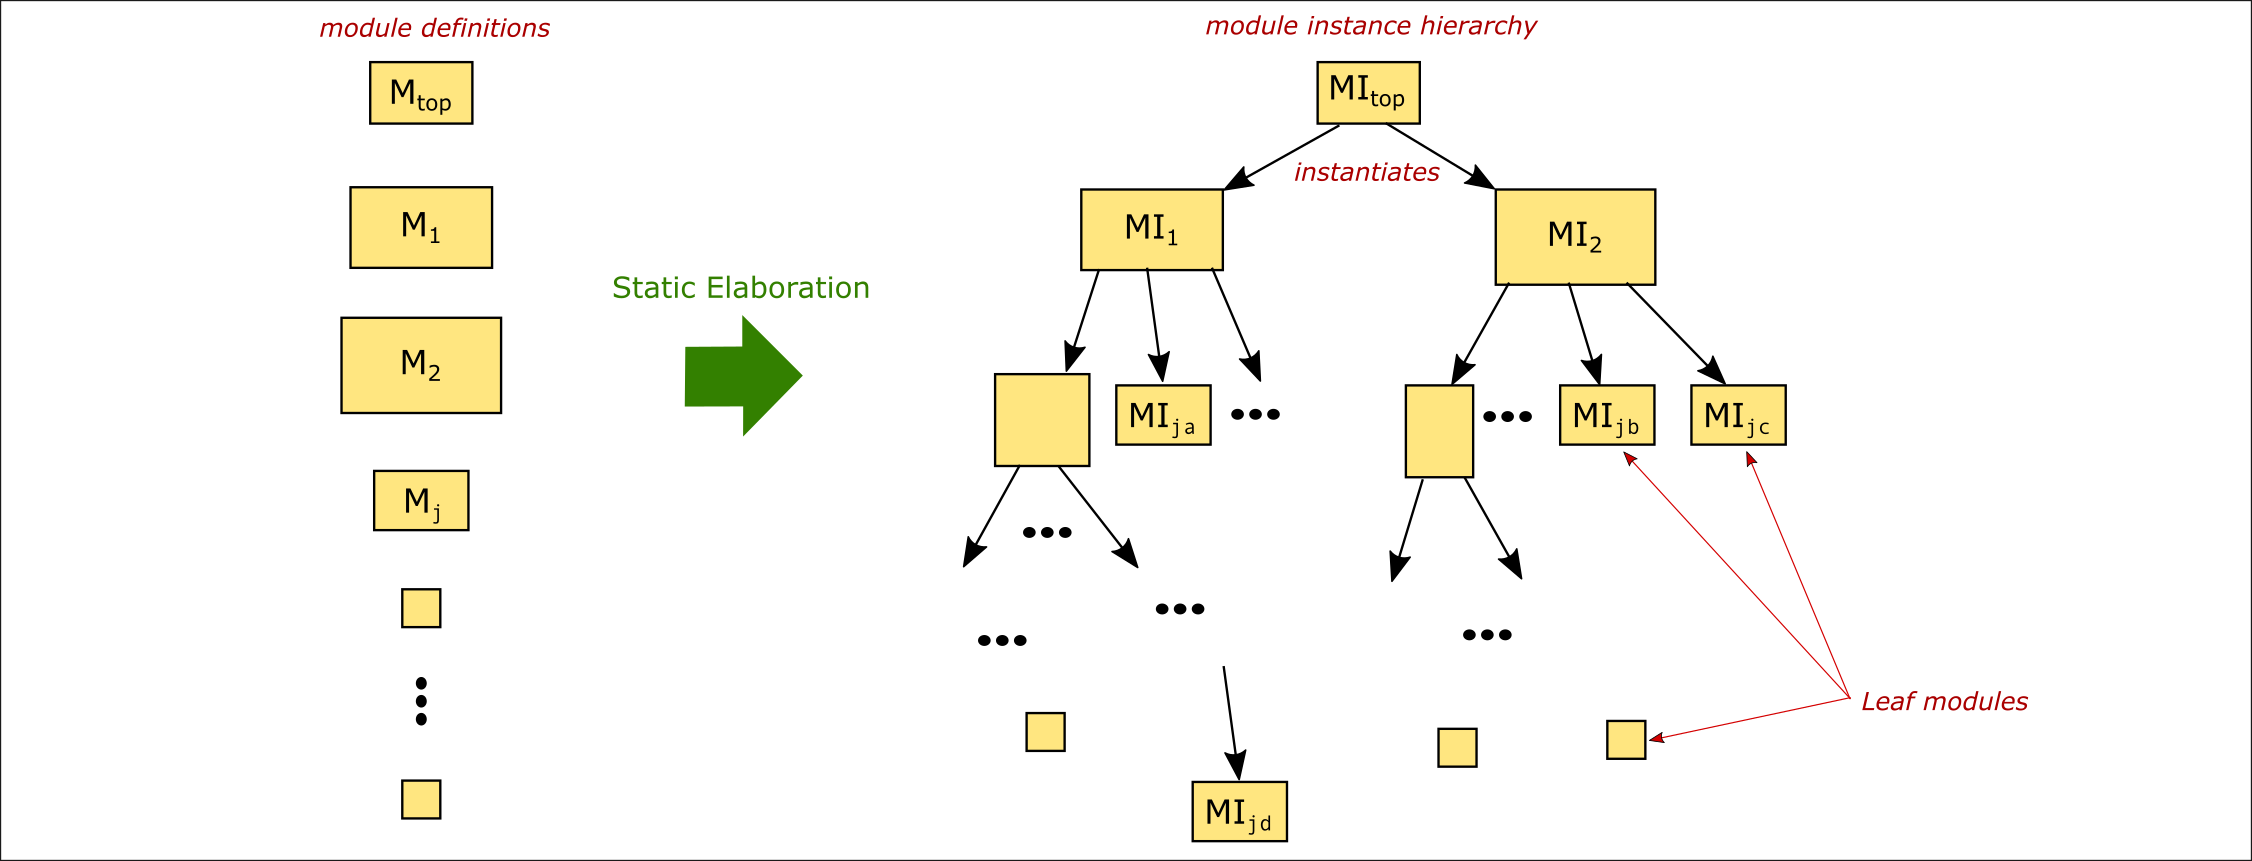
\includegraphics[width=\textwidth]{../Figures/Fig_BSV_static_elaboration}
\end{center}

\end{frame}

% ================================================================

\begin{frame}
\frametitle{Module interaction}

\begin{center}

\includegraphics[width=\textwidth]{../Figures/Fig_BSV_module_interaction}
\end{center}

\end{frame}

% ================================================================

% -*- mode: fundamental -*-

% Slides accompanying "Learn RISC-V CPU Implementation and BSV" book
% Copyright (c) 2024 Rishiyur S. Nikhil, All Rights Reserved

% This is a postamble shared by all the slide decks

% ================================================================

\begin{frame}

\begin{center}
  {\LARGE End}
\end{center}

\end{frame}

% ================================================================


% ****************************************************************

\end{document}
